\documentclass[
  captions=tableheading,
  bibliography=totoc, 
  titepage=firstiscover,
]{scrartcl}

\usepackage{blindtext} %neuer input

\usepackage{longtable} % Tabellen über mehrere Seiten

\usepackage[utf8]{inputenc} %neuer input

\usepackage{scrhack}

\usepackage[aux]{rerunfilecheck} %Warnung falls nochmal kompiliert werden muss

\usepackage{fontspec} %Fonteinstellungen

\recalctypearea{}

\usepackage[main=ngerman]{babel} %deutsche Spracheinstellung

\usepackage{ragged2e} %neuer input

\usepackage{amsmath, nccmath}

\usepackage{amssymb} %viele mathe Symbole

\usepackage{mathtools} %Erweiterungen für amsmath


\DeclarePairedDelimiter{\abs}{\lvert}{\rvert}
\DeclarePairedDelimiter{\norm}{\lVert}{\rVert}

\DeclarePairedDelimiter{\bra}{\langle}{\rvert}
\DeclarePairedDelimiter{\ket}{\lvert}{\rangle}

\DeclarePairedDelimiterX{\braket}[2]{\langle}{\rangle}{
#1 \delimsize| #2
}

\NewDocumentCommand \dif {m}
{
\mathinner{\symup{d} #1}
}


\usepackage[
  math-style=ISO,
  bold-style=ISO,
  sans-style=italic,
  nabla=upright,
  partial=upright,
  warnings-off={
    mathtools-colon,
    mathtools-overbracket,
  },
]{unicode-math}

\setmathfont{Latin Modern Math}
\setmathfont{XITS Math}[range={scr, bfscr}]
\setmathfont{XITS Math}[range={cal, bfcal}, StylisticSet=1]


\usepackage[
  locale=DE,
  separate-uncertainty=true,
  per-mode=reciprocal,
  output-decimal-marker={,},
]{siunitx}

\usepackage[autostyle]{csquotes} %richtige Anführungszeichen

\usepackage{xfrac}

\usepackage{float}

\floatplacement{figure}{htbp}

\floatplacement{table}{htbp}

\usepackage[ %floats innerhalb einer section halten
  section,   %floats innerhalb er section halten
  below,     %unterhalb der Section aber auf der selben Seite ist ok
]{placeins}

\usepackage[
  labelfont=bf,
  font=small,
  width=0.9\textwidth,
]{caption}

\usepackage{subcaption} %subfigure, subtable, subref

\usepackage{graphicx}

\usepackage{grffile}

\usepackage{booktabs}

\usepackage{microtype} %Verbesserungen am Schriftbild

\usepackage[
backend=biber,
]{biblatex}

\addbibresource{../lit.bib}

\usepackage[ %Hyperlinks im Dokument
  german,
  unicode,
  pdfusetitle,
  pdfcreator={},
  pdfproducer={},
]{hyperref}

\usepackage{bookmark}

\usepackage[shortcuts]{extdash}

%\usepackage{warpcol}

\allowdisplaybreaks

\begin{document}
    \title{Physik IV Übungsblatt 4}
    \author{  
    Tobias Rücker\\
    \texorpdfstring{\href{mailto:tobias.ruecker@tu-dortmund.de}{tobias.ruecker@tu-dortmund.de}
    \and}{,} 
    Paul Störbrock\\
    \texorpdfstring{\href{mailto:paul.stoerbrock@tu-dortmund.de}{paul.stoerbrock@tu-dortmund.de}}{}
    }
\maketitle
\center{\Large Abgabegruppe: \textbf{4H}}
\thispagestyle{empty}

\newpage
\tableofcontents
\thispagestyle{empty}
\newpage

\setcounter{page}{1}

\section{Aufagabe 1}

    \begin{figure}[H]
        \centering
        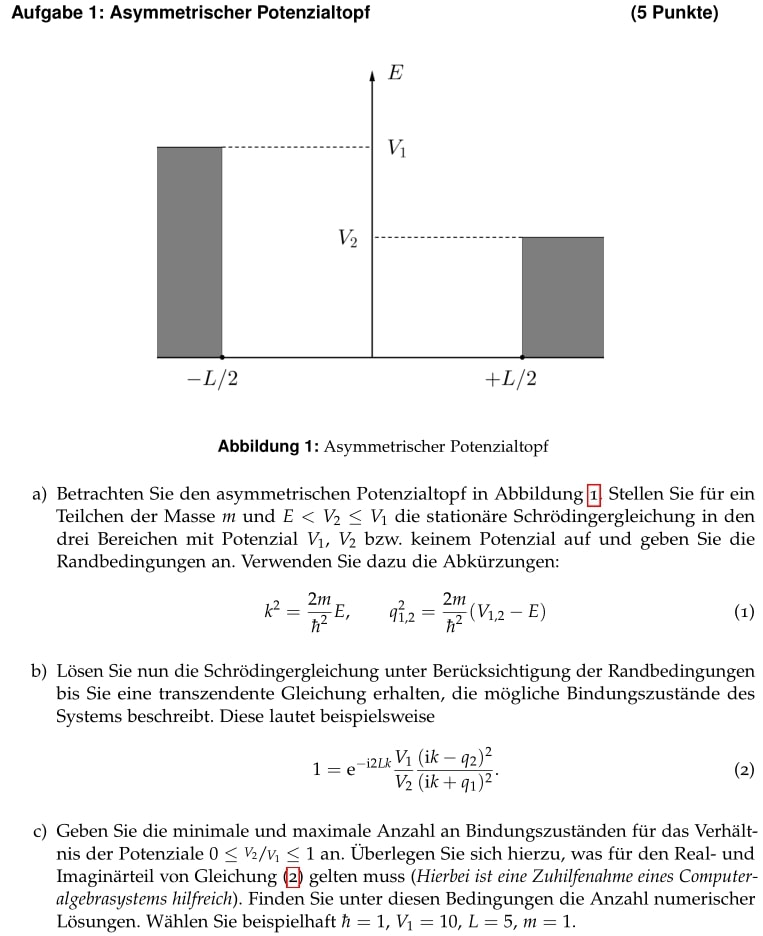
\includegraphics[width=\linewidth]{images/Aufgabe1.jpg}
        \label{fig:1}
    \end{figure}

    \subsection{a)}

    Fall $V=V_{1,3} \; \text{und} \; \abs{x}> \frac{L}{2} $:

    \begin{align*}
    E \varphi_{1,3} (x) &=-\frac{\hbar^2}{2m} \frac{\partial ^2 \varphi _{1,3} (x)}{\partial x^2}+ V_{1,2} (x) \varphi _{1,3}(x)\\
    \frac{\partial ^2 \varphi _{1,3}}{\partial x^2} &= \-- \frac{2m}{\hbar ^2} (E-V_{1,2})\varphi _{1,3}\\
    &= q_{1,2}^2 \varphi _{1,3}\\
    \varphi _1 (x)&=A e^{q_1x}+A' e^{-q_1 x}\\
    \varphi _3 (x)&=B e^{q_2x}+B' e^{-q_2 x}\\
    \intertext{
        Fall $V=0 \; \text{und} \; \abs{x} \leq \frac{L}{2} $:
    }
    \frac{\partial ^2 \varphi _3(x)}{\partial x^2} &=-\frac{2m}{\hbar ^2}E \varphi _3(x)\\
    &=-k^2 \varphi _3\\
    \varphi _2 &= C e^{ikx}+C' e^{-ikx}
    \intertext{
        Randbedingungen
        $\varphi _1$ muss normierbar sein für  $\lim_{x \to -\infty} \varphi _1 (x) \ne \infty$ 
    }
    \Rightarrow A'&= 0
    \intertext{
        Das gleiche gilt für $\varphi _3 $ für $\lim_{x \to \infty} \varphi _3 \ne \infty $.
    }
    \Rightarrow B &= 0
    \intertext{
        Stetigkeitsbedingungen an der linken Wand
    }
    \end{align*}
    \begin{align*}    
    \varphi _1 \left(-\frac{L}{2}\right)&= \varphi_2 \left(-\frac{L}{2}\right)\\
    A e^{-q_1 \frac{L}{2}}&=B e^{-q_2\frac{L}{2}}+A' e^{q_2 \frac{L}{2}}\\
    &\text{\noindent\makebox[\linewidth]{\rule{\linewidth}{0.4pt}}}\\
    \frac{\partial \varphi _1}{\partial x } \vert _{x=-\frac{L}{2}} &=\frac{\partial \varphi _2}{\partial x } \vert _{x=-\frac{L}{2}}\\ 
    A e^{-q_1 \frac{L}{2}} &= ik C e^{-ik \frac{L}{2}}-ik C' e^{ik \frac{L}{2}}\\
    &\text{\noindent\makebox[\linewidth]{\rule{\linewidth}{0.4pt}}}\\
    \intertext{
        Stetigkeitbedingungen an der rechten Wand
    }
    \varphi_2 \left(\frac{L}{2} \right) &= \varphi _3 \left(\frac{L}{2} \right)\\
    C e^{i k \frac{L}{2}} + C' e^{-i k \frac{\L}{2}} &= B' e^{-q_2 \frac{L}{2}}\\
    \frac{\partial \varphi _2}{\partial x} \vert _{x=\frac{L}{2}} &= \frac{\partial \varphi _3}{\partial x} \vert _{x=\frac{L}{2}}\\
    i k C e^{ik \frac{L}{2}}-ik C' e^{-ik \frac{L}{2}} &= \-- q_2 B' e^{-q_2 \frac{L}{2} }
    \end{align*}

    \flushleft{Die\,}\justifying vier Gleichungen für die 4 Paramter A, C, C' und B' bilden ein
    homogenes Gleichungssystem. Da das System eindeutige Lösungen besitzen muss,
    muss die Säkulardeterminante 0 ergeben.
    \subsection{b)}
$
    \begin{vmatrix}
        e^{-q_1 \frac{L}{2}} & -e^{-ik \frac{L}{2}} & -e^{ik\frac{L}{2}} & 0\\
        0 & e^{ik \frac{L}{2}} & e^{-ik\frac{L}{2}}  & -e^{-q_2 \frac{L}{2}}   \\
        q_1 e^{-q_1 \frac{L}{2}} & -ik e^{-ik \frac{L}{2}} & ik e^{ik \frac{L}{2}} & 0  \\
        0 & ik e^{ik \frac{L}{2}} & -ik e^{-ik \frac{L}{2}} & q_2 e^{-q_2 \frac{L}{2}}  
    \end{vmatrix}
    =0
$

$
e^{-q-1 \frac{L}{2}}
\begin{vmatrix}
  e^{ik \frac{L}{2}}  & e^{-ik \frac{L}{2}} & - e^{-q_2 \frac{L}{2}}\\
  -ik e^{-ik\frac{L}{2}}  & ik e^{ik\frac{L}{2}} & 0\\
  ik e^{ik\frac{L}{2}}  & -ik e^{-ik \frac{L}{2}}  & q_2 e^{- q_2 \frac{L}{2}}
\end{vmatrix}
+ e^{-ik\frac{L}{2}}
\begin{vmatrix}
 0  & e^{-ik \frac{L}{2}} & - e^{-q_2 \frac{L}{2}}\\
  q_1 e^{-q_1 \frac{L}{2}} & ik e^{ik \frac{L}{2}} & 0 \\
 0  & -ik e^{-ik \frac{L}{2}} & q_2 e^{-q_2 \frac{L}{2}} 
\end{vmatrix}\\
-e^{ik\frac{L}{2}}
\begin{vmatrix}
 0  &  e^{ik \frac{L}{2}} & -e^{-q_2 \frac{L}{2}} \\   
 q_1 e^{-q_1 \frac{L}{2}}  & -ik e^{-ik \frac{L}{2}}  & 0   \\
 0  &  ik e^{ik \frac{L}{2}} & q_2 e{-q_2 \frac{L}{2}}   
\end{vmatrix}
+0 = 0 
$

\begin{align*}
    &e^{-q_1 \frac{L}{2}}\left(ik q_2 e^{ikL-q-2 \frac{L}{2}}+ k^2 e^{-q_2 \frac{L}{2} -ikL}+ikq_2 e^{-ikL -q_2 \frac{L}{2}}
    - k^2 e^{ikL-q_2 \frac{L}{2}} \right)\\
     &+ e^{-ik \frac{L}{2}} \left(ik q_1 e^{-ik \frac{L}{2}-q_2\frac{L}{2}-q_1\frac{L}{2}}
    -q_1 q_2 e^{-ik\frac{L}{2}-q_1 \frac{L}{2}-q_2 \frac{L}{2}} \right)\\
    &-e^{ik\frac{L}{2}}\left( 
        -ikq_1 e^{-q_2 \frac{L}{2}-q_1\frac{L}{2} +ik \frac{L}{2} }-q_1 q_2 e^{-q-1\frac{L}{2} -q_2\frac{L}{2} +ik \frac{L}{2}} \right)=0\\
        &0= (ik q_2 -k^2+ ik q_1 +q_1 q_2) e^{-q_2 \frac{L}{2} - q_1 \frac{L}{2} +ikL }
        +(ikq_2 + k^2 +ikq_1 -q_1 q_2) e^{-ikL-q_1 \frac{L}{2} - q_2 \frac{L}{2}}\\
    &-\frac{ikq_2 + k^2 + ik q_1 -q_1 q_2}{ik q_2 - k^2 + ik q_1 + q_1 q_2} e^{-i2Lk} = 1\\
    &1= e^{-i2Lk} \frac{(q_2-ik)(q_1-ik)}{(q_1 + ik)(q_2+ik)}\\
    \intertext{Nebenrechnung}
    & q_{1,2}^2 = \frac{2m}{\hbar ^2} (V_{1,2}-E )\\
    & V_{1,2} = \frac{\hbar ^2}{2m} q_{1,2}^2+E\\
    &E= \frac{\hbar ^2 k^2}{2m}\\
    &\to V_{1,2} = \frac{\hbar ^2}{2m} q_{1,2}^2+\frac{\hbar ^2 k^2}{2m}\\
    &\frac{V_1}{V_2}= \frac{q_1^2 +k^2}{q_2^2 +k^2} =\frac{(q_1 +ik)(q_1-ik)}{(q_2+ik)(q_2-ik)}\\
    & \frac{V_1}{V_2} \frac{q_2-ik}{q_1+ik} = \frac{q_1-ik}{q_2 +ik}\\
    \intertext{Ende Nebenrechnung}
    & \Rightarrow 1 = e^{-i2kL} \frac{V_1}{V_2} \frac{(ik-q_2)^2}{(ik+q_1)^2}
\end{align*}

    \subsection{c)}
    \flushleft{In\,}\justifying der vorherigen Gleichung wird der komplexe Bruch in 
    Schreibweise der Euler-Formel umgeschrieben mit
    \begin{align*}
        \varphi &= \arctan \left(\frac{b}{a} \right) b>0 \hat a>0 (z = a+ib)\\
        \varphi &= \arctan \left(\frac{b}{a} \right) + \pi b>0 \hat a<0\\
        \abs{z} &= \sqrt{a^2+b^2}\\
        1&= e^{-i2kL} \frac{V_1}{V_2}  \frac{(k^2+q_2^2) e^{2i(\arctan \left(\frac{k}{q_2}+\pi \right) )}}{(k^2+q_1^2) e^{2i \arctan \left(\frac{k}{q_1} \right)} }\\
        \intertext{
            \flushleft{Diese\,}\justifying Gleichung ist erfüllt, wenn Winkelanteil und Betrag auf beiden Seiten der Gleichung
            identisch sind.
        }
        \frac{V_1}{V_2}\frac{k^2+q_2^2}{k^2+q_1^2}&=1\\
        1&=1\\
        -2kL + 2 \arctan \left(\frac{q_2}{k} \right) &-2 \arctan \left(\frac{q_1}{k}+2 \pi=2 \pi n \right)\\
        \intertext{
            Die Lösung erfolgt allerdings mit der Exponential-Gleichung. Es wird q und k
            eingesetzt sowie die vorgegebenen Werte. Das ganze wird dann graphisch ausgewertet,
            indem die Nullstellen gezählt werden.
        }
        \frac{k}{q_{1,2}}&= \sqrt{\frac{E}{V_{1,2}-E}}\\
        \hbar &= m=1\; L=5\; V_1=10
    \end{align*}
    \[
        f(E)=\exp\left(i2\left(\--5 \sqrt{2E}+ \arctan \left(\sqrt{\frac{E}{V_2 -E}} \right) +\pi -\arctan \left(\sqrt{\frac{E}{10-E}} \right)\right)\right)-1
    \] 

\section{Aufgabe 2}

    \begin{figure}[H]
        \centering
        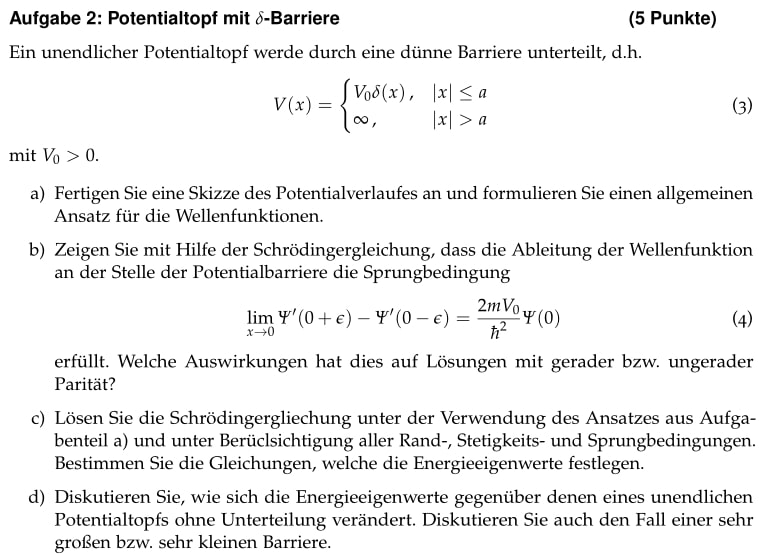
\includegraphics[width=\textwidth]{images/Aufgabe2.jpg}
        \label{fig:2}
    \end{figure}

    \subsection{a)}

    \begin{figure}[H]
        \centering
        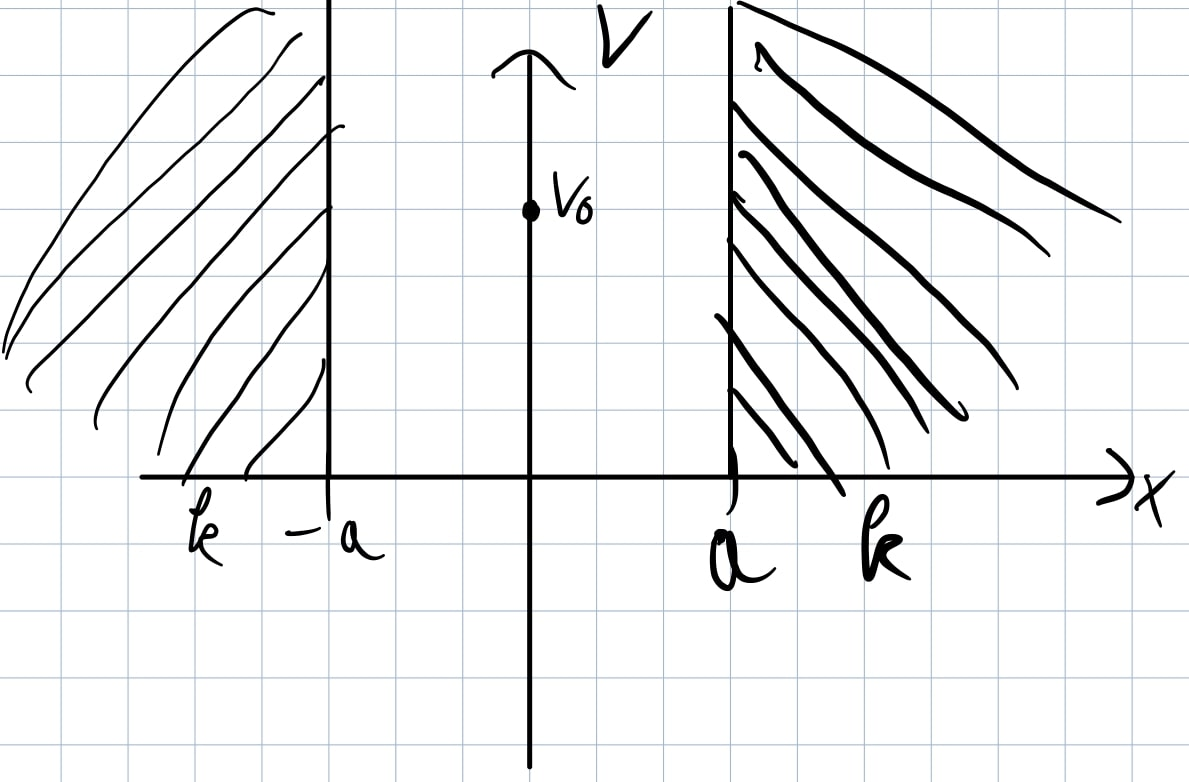
\includegraphics[width=\textwidth]{images/2a.jpg}
        \label{fig:3}
    \end{figure}

    \begin{align*}
        \intertext{Bereich $a \leq x \leq 0$:
        }
        \varphi_1(x) &= A\sin(kx) + A'\cos(kx)
        \intertext{Bereich $0 \leq x \leq a$:
        }
        \varphi_2(x) &= B\sin(kx) + B'\cos(kx)\\
        \varphi(x) &= 0 \qquad \text{sonst}
    \end{align*}

    \subsection{b)}

    \begin{align*}
        -\frac{\hbar^2}{2m} \frac{\partial^2 \varphi(x)}{\partial x^2} + V(x)\varphi(x) &= E\varphi(x) \qquad \vert \int_{-\epsilon}^{\epsilon}\,\mathrm{d}x\\
        \lim_{\epsilon \to 0} \left( \int_{-\epsilon}^{\epsilon} -\frac{\hbar^2}{2m} \frac{\partial^2 \varphi(x)}{\partial x^2} \mathrm{d}x + V_0\,\delta(x)\,\varphi(x) \mathrm{d}x \right) &= \underbrace{\lim_{\epsilon \to 0} \int_{-\epsilon}^{\epsilon} E\,\varphi(x) \mathrm{d}x}_{=0}
        \intertext{\flushleft{Das\;}\justifying Integral über eine Fläche mit endlicher Höhe und infinitesimal schmaler Breite ist 0.
        }
        \lim_{\epsilon \to 0} \left[ -\frac{\hbar^2}{2m} \frac{\partial \varphi(x)}{\partial x} \right]_{-\epsilon}^{\epsilon} + V_0\,\varphi(0) &= 0\\
        \Leftrightarrow \lim_{\epsilon \to 0} \varphi'(0+\epsilon) - \varphi'(0-\epsilon) &= \frac{2m}{\hbar^2} V_0\,\varphi(0)
        \intertext{\flushleft{Für\;}\justifying ungerade Parität gilt:
        }
        \varphi(x) &= -\varphi(-x)\\
        \varphi'(x) &= \varphi'(-x)\\
        \lim_{\epsilon \to 0} \varphi'(\epsilon) - \varphi'(-\epsilon) &= 0
        \intertext{\flushleft{Für\;}\justifying gerade Parität gilt:
        }
        \varphi(x) &= \varphi(-x)\\
        \varphi'(x) &= -\varphi'(-x)\\
        \lim_{\epsilon \to 0} \varphi'(\epsilon) - \varphi'(-\epsilon) &= \lim_{\epsilon \to 0} 2\varphi'(\epsilon)
    \end{align*}

    \subsection{c)}

    \begin{align*}
        \varphi_1(x) &= A\sin(kx) + A'\cos(kx)\\
        \varphi_2(x) &= B\sin(kx) + B'\cos(kx)\\
        \varphi(x) &= 0 \qquad \text{sonst}
        \intertext{\flushleft{Fall\;}\justifying 1:
        }\\
        \varphi_1(-a) &= -\varphi_2(a) = 0\\
        \lim_{\epsilon \to 0} \varphi'(\epsilon) - \varphi'(-\epsilon) &= 0 = \frac{2m}{\hbar^2} V_0\,\varphi(0)\\
        \varphi_1'(0) &= \varphi_2'(0)\\
        \Leftrightarrow A' &= B'\\
        \varphi(0) &= 0\\
        \Rightarrow A' &= 0 \qquad B' = 0\\
        \varphi_1(-a) &= -\varphi_2(a)\\
        A\sin(-ka) &= -B\sin(ka)\\
        \Leftrightarrow -A\sin(ka) &= -B\sin(ka)\\
        \Leftrightarrow A &= B\\
        &\varphi(x)\begin{cases}
            A\sin(kx)\; \text{für}\; -a\leq x\leq 0\\
            A\sin(kx)\; \text{für}\; 0 \leq a
        \end{cases}\\
        \Rightarrow \varphi(x) &= A\sin(kx) \qquad x\leq a\\
        \varphi(-a) &= 0\\
        \Leftrightarrow A\sin(-ka) &= 0\\
        \Rightarrow ka &=\pi n\\
        \Leftrightarrow k &= \frac{\pi n}{a} \qquad n \in \mathbb[Z]\\
        k &= \frac{\sqrt{2mE}}{\hbar}\\
        \Rightarrow \frac{\pi n}{a} &\stackrel{!}{=}  \frac{\sqrt{2mE_n}}{\hbar}\\
        \Leftrightarrow E_n &= \frac{\pi^2 \hbar^2}{2m a^2}n^2
        \intertext{\flushleft{Fall\;}\justifying 2:
        }\\
        \varphi_1(-a) &= \varphi_2(a) = 0\\
        \lim_{\epsilon \to 0} \varphi_2'(\epsilon) - \varphi_1(-\epsilon) &= \frac{2mV_0}{\hbar^2} \varphi(0)\\
        &= \varphi_1(0) = \varphi_2(0)\\
        \Rightarrow A' &= B' \tag{*}\\
        \varphi_1(-a) &= \varphi_2(a)\\
        A\sin(-ka) + A'\cos(-ka) &= B\sin(ka) + B'\cos(ka) \\
        -A\sin(ka) + \underbrace{A'\cos(ka)}_{wegk"urzen} &\stackrel{(*)}{=} B\sin(ka) + \underbrace{A'\cos(ka)}_{wegk"urzen}\\
        \Rightarrow -A &= B\\
        \frac{2mV_0}{\hbar^2}A' &= \lim_{\epsilon \to 0} \left( -kA\cos(k\epsilon) - kA'\sin(k\epsilon) - kA\cos(-k\epsilon) + A'\sin(-k\epsilon) \right) \\
        \Leftrightarrow kA - kB &= A'\frac{2mV_0}{\hbar^2}\\
        \Leftrightarrow -2kA &= A'\frac{2mV_0}{\hbar^2}\\
        -\frac{A}{A'} &= \frac{2mV_0}{k\hbar^2}\\
        \varphi_1(-a) &= 0\\
        A\sin(-ka) + A'\cos(-ka) &= 0\\
        \frac{A}{A'} &= \cot(ka)\\
        -\cot(ka) &\stackrel{!}{=} \frac{mV_0}{k\hbar^2} \qquad z=ka\\
        \cot(z) &= \frac{mV_0}{\hbar^2} \frac{1}{z}a \qquad \text{numerisch lösbar}\\
        \Rightarrow z &= ka = a \cdot \frac{\sqrt{2mE}}{\hbar}\\
        \Leftrightarrow E &= \frac{\hbar^2}{2m} \left( \frac{z}{a} \right)^2
    \end{align*}

    \subsection{d)}

    \begin{align*}
        \intertext{\flushleft{Lösung\;}\justifying für den unendlichen Potentialtopf:
        }
        E_n &= \frac{n^2 \hbar^2 \pi^2}{2ma^2}
        \intertext{Ungerade:
        }
        E_n &= \frac{n^2 \hbar^2 \pi^2}{2ma^2} \qquad \text{identisch}
        \intertext{Gerade:
        }
        E &= \frac{\hbar^2}{2m} \left( \frac{z}{a} \right)^2
        \intertext{\flushleft{Werden\;}\justifying die beiden Lösungen verglichen, fällt auf, dass die gerade Lösung des unendlichen Potentialtopfs
        nur eine Teilmenge der Gesamtlösung ist.
        }
        \intertext{\flushleft{Grenzfälle}\justifying:
        }
        \intertext{$V_0 \to \infty$
        }
        -\cot(ka) &= \frac{mV_0}{k\hbar^2}\\
        \Leftrightarrow \tan(ka) &= -\frac{k\hbar^2}{mV_0}\\
        \Rightarrow \tan(ka) &= 0\\
        \Rightarrow ka &= n\pi\\
        \Rightarrow E_n &= \frac{\hbar^2}{2m} \frac{n^2\pi^2}{a^2}
        \intertext{\flushleft{Unendlicher\;}\justifying Potentialtopf ohne Barriere:
        }
        \intertext{$V_0 \to 0$
        }
        \tan(ka) &= -\frac{k\hbar^2}{mV_0} \to -\infty\\
        ka &= \pi\left( \frac{1}{2}+c \right) \qquad c \in \mathbb{Z}\\
        \Leftrightarrow k &= \frac{\pi}{a}\left( \frac{1}{2}+c \right)\\
        \frac{\pi}{a}\left( \frac{1}{2}+c \right) &\stackrel{!}{=} \frac{\sqrt{2mE}}{\hbar}\\
        \Leftrightarrow E &= \frac{\pi^2}{a^2}\frac{\hbar^2}{2m} \left( \frac{1}{2}+c \right)^2
    \end{align*}

\section{Aufgabe 3}

    \begin{figure}[H]
        \centering
        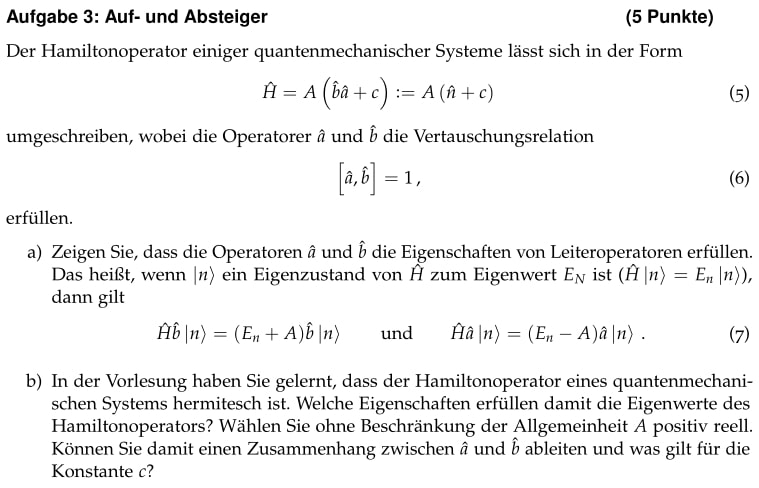
\includegraphics[width=\textwidth]{images/Aufgabe3ab.jpg}
        \label{fig:4}
    \end{figure}
    \begin{figure}[H]
        \centering
        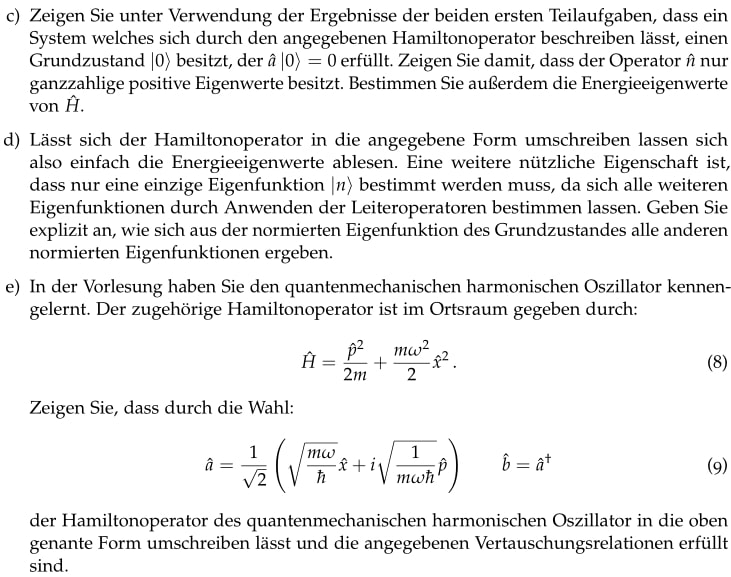
\includegraphics[width=\textwidth]{images/Aufgabe3cde.jpg}
        \label{fig:5}
    \end{figure}

    \subsection{a)}

    \begin{align*}
        \hat{H} &= A\left( \hat{b}\hat{a} + c \right)\\
        \left[ \hat{a}, \hat{b} \right] &= 1\\
        \Rightarrow \hat{a}\hat{b} - \hat{b}\hat{a} &= 1\\
        \Leftrightarrow \hat{a}\hat{b} &= \hat{b}\hat{a} + 1\\
        \Leftrightarrow \hat{b}\hat{a} &= \hat{a}\hat{b} - 1\\
        \\
        \hat{H}\hat{b} \vert n \rangle &= A\left( \hat{b}\hat{a} +c \right)\hat{b} \vert n \rangle\\
        &= A\left(\hat{b}\hat{a}\hat{b}+c\hat{b} \right) \vert n \rangle\\
        &= A\hat{b} \left( \underline{\hat{a}\hat{b}} +c \right) \vert v \rangle\\
        &= A\hat{b} \left( \underline{\hat{b}\hat{a} + 1} + c \right) \vert n \rangle\\
        \Leftrightarrow &= \hat{b} \left(\underbrace{A\left(\hat{b}\hat{a}+c \right)}_{=\hat{H}} + A \right) \vert n \rangle\\
        &= \hat{b} \left( \hat{H} + A \right) \vert n \rangle\\
        &= \left( E_N + A \right) \hat{b} \vert n \rangle\\
        \\
        \hat{H}\hat{a} \vert n \rangle &= A\left( \hat{b}\hat{a} +c \right)\hat{a} \vert n \rangle\\ 
        &= A\left(\underline{\hat{b}\hat{a}}\hat{a}+c\hat{a} \right) \vert n \rangle\\
        &= A\left( \underline{\left( \hat{b}\hat{a}-1  \right)} \hat{a} + c\hat{a} \right)\vert n \rangle\\
        \Leftrightarrow &= A\hat{a} \left( \hat{b}\hat{a} - 1 + c \right) \vert n \rangle\\
        \Leftrightarrow &= \hat{a} \left(\underbrace{A\left(\hat{b}\hat{a}+c \right)}_{=\hat{H}} - A \right) \vert n \rangle\\
        &= \hat{a} \left( \hat{H} - A \right) \vert n \rangle\\
        &= \left( E_N - A \right) \hat{a} \vert n \rangle
    \end{align*}

    \subsection{b)}

    \subsection{c)}

    \subsection{d)}

    \subsection{e)}

\end{document}